\chapter{Introducción}
\pagenumbering{arabic}
\setcounter{page}{1}
%\renewcommand{\baselinestretch}{2} %doble espacio paratodo el texto
%\renewcommand{\baselinestretch }{1.5}

Las empresas para elaborar sus planes de mercadeo y su planeación requieren la elaboración inicial de un pronóstico de ventas, el cual les permitirá proyectar las posibles ventas futuras basándose
en datos históricos de la misma empresa, con el fin de planear, administrar y controlar los presupuestos necesarios para un buen uso de los recursos que se requerirán para cumplir con las metas propuestas.

El pronóstico de ventas es una herramienta comercial que permite estimar las ventas a futuro, con el fin de establecer metas en un determinado periodo, para su elaboración se tienen en cuenta los resultados históricos y las tendencias de ventas presentadas por el área comercial.

En base a eso, la empresa (restaurant Combiche-Trujillo), mediante sus datos históricos de ventas, desea conocer cuáles serán las ventas que obtendrán en los siguientes periodos posterior a su
análisis. Con el apoyo de las redes neuronales, se busca estimar las ganancias que se obtendrán según el número de ventas pronosticadas , dado que en la actualidad, existen varios restaurantes en la ciudad de Trujillo, y que gracias a la aplicación de dicha herramienta computacional, contribuirá a que la empresa tome medidas de precaución cuando el mercado esté bajo.

\section{Justificación de la investigación}
La importancia de esta investigación desde un punto de vista informático se justifica académicamente, como un aporte para la investigación y una motivación para profundizar en inteligencia artificial, redes neuronales.

Este proyecto se justifica socialmente, ya que no solo beneficiará a la empresa, restaurant Combiche - Trujillo, sino a los comensales que desean degustar las variedades de platos que estan a la venta, y al ser realizado con sistemas basado en conocimiento mediante RNA la aplicación irá mejorando a medida que se vaya usando en el pronóstico de las ventas, ya que tiene la principal ventaja de ir aprendiendo.

\section{Formulación del problema}
El problema de la empresa es establecer medidas de precaución ante las bajas ventas que se puedan tener y para ello se necesita de una herramienta computacional que pronostique, en base a las ventas históricas de la empresa, si hay ganancias o pérdidas de las ventas para tomar una decisión que beneficie a la empresa. Analizando nuestro problema, nos nace la siguiente pregunta:
 
 \begin{center} 
     ¿Cómo pronosticar las ventas de un producto utilizando una red neuronal artificial?
 \end{center}

\section{Hipótesis}
Mediante el desarrollo de un sistema basado en conocimiento utilizando R.N.A. se podrá pronosticar las ventas en el Mall Aventura Plaza.




\section{Objetivos}
\subsection{Generales}
Desarrollar un sistema basado en conocimiento mediante RNA para pronosticar las ventas de un producto.
\subsection{Específicos}
\begin{itemize}
\item Realizar una investigación bibliográfica para recolectar datos referentes al tema de investigación y analizar los resultados de una encuesta aplicada a un experto en ventas.
\item Aplicar la metodología RUP para sistemas basados en conocimientos.
\item Diseñar la arquitectura de nuestro sistema basado en conocimiento.
\item Entrenar el software basándonos en el modelo computacional diseñado previamente.
\item Analizar los resultados obtenidos con el software.
\end{itemize}

\section{Estructura de la tesis}

En presente trabajo de investigación tiene los siguientes capítulos:

\begin{itemize}
 \item En el primer capítulo se desarrolla los aspectos generales así como la justificación, formulación del problema, hipótesis de la investigación y  objetivos del presente trabajo de investigación.
 \item En el segundo capítulo se realiza la recopilación de diferentes conceptos y definiciones que es de mucha importancia a lo largo de toda la investigación, como la metodología de investigación, inteligencia artificial, sistemas inteligentes, redes neuronales, perceptrón, perceptrón multicapa, backpropagation. También se define el vector característico, la extracción de datos y por último como conceptos finales, consideramos a los gestores, plataformas y lenguajes de programación que utilizaremos así como Visual Studio Code, Tensorflow, Python.
 \item En el tercer capítulo se analiza, comprende, implementa  y optimiza las soluciones de los sistemas inteligentes para la clasificación automática de documentos. Empezando por algunos problemas de algoritmos actuales. También la prueba a seguir de redes neuronales, se diseñan los modelos propuestos y se explica la implementación del sistema.
 \item En el cuarto capítulo se contrasta los resultados con el prototipo de la aplicación de sistemas inteligentes para la clasificación automática de documentos.
 \item En el quinto capítulo se presenta las conclusiones de nuestro trabajo de investigación, demostrando los objetivos cumplidos.
\end{itemize}




\chapter{Materiales y Métodos}
\renewcommand{\baselinestretch}{2} %doble espacio paratodo el texto}

\section{Marco teórico}
El siguiente capítulo presenta conceptos importantes que utilizamos como parte fundamental para el desarrollo de nuestra tesis, este material bibliográfico fue investigado por la relación que tiene con los temas de nuestra investigación. La investigación se tornó muy amplia, principalmente en los conceptos claves para nuestro conocimiento científico, el cual ayudó a desarrollar la tesis, inteligencia artificial, sistemas inteligentes, redes neuronales, perceptrón, backpropagation, conceptos importantes ya que sin ellos sería imposible el modelamiento y desarrollo.

\subsection{Inteligencia Artificial (IA)}
Empecemos esto con una pregunta clave: ¿Qué es la inteligencia artificial?. Aunque es un término de compleja definición, esta puede ser catalogada como una rama de la ciencia que se dedica al estudio de la forma en que se desarrolla el proceso del pensamiento humano para reproducirlo en un ente artificial. Es por ello que para poder lograrlo, la I.A. centra su estudio en dos áreas: el cuerpo humano (estudio de la inteligencia) y el ordenador electrónico. Teniendo en cuenta que para poder reproducir el pensamiento es necesario conocerlo, como primera meta para la investigación de los científicos fue entender los procesos cognoscitivos de la mente humana. De esta manera definir su modelo de inteligencia, para luego proceder a programarlo en ordenadores, simulando cada uno de los procesos y comprobando los resultados de sus teorías. \citep{Belzebu2009}. 

Según \cite{mccarthy1989artificial}, acuñó la expresión ``inteligencia artificial'', y la definió como: ``la ciencia e ingenio de hacer máquinas inteligentes, especialmente programas de cómputo inteligentes''.

\subsection{Sistemas inteligentes}
Los sistemas inteligentes radican en un conjunto de herramientas y aplicaciones que agrupados llevan a cabo la recopilación, extracción y formato de información obtenida de distintas fuentes con el único propósito de crear medios inteligentes y artificiales para múltiples usos. Frecuentemente se usa para el soporte en la toma de decisiones, sin embargo, esta no es su única funcionalidad.\\
Son sistemas que, durante su existencia, aprenden y almacenan para luego actuar continuamente de forma interna o externa, de forma que pueda alcanzar su propósito superándose cada vez. Tiene su propio objetivo esencial y para alcanzarlo, escoge una acción tomada de las experiencias que   ha almacenado en su memoria.

Para poder hablar de un sistema inteligente es necesario que exista un entorno con el cual el sistema pueda interactuar y, además, el sistema inteligente debe contener ``sentidos'' que le permitan recibir comunicaciones de dicho entorno y con ello poder transmitir información. El sistema actúa continuamente   y cuenta con una memoria para archivar el resultado de sus acciones. 
Como se dijo anteriormente, este sistema tiene un objetivo, por lo cual, el conseguirlo significaría el hecho de seleccionar la respuesta adecuada ante cada estimulo. También se caracteriza porque a través de su memoria, durante su existencia, aprende de sus experiencias, logrando así, mejorar tanto su rendimiento como su eficiencia. Por último, es necesario indicar que este sistema consume energía, la cual   utiliza en sus procesos internos y su actuar. \citep{Alejandro2017}.

\subsubsection{Capacidades requeridas}
Según \cite{Alejandro2017}, un sistema inteligente podrá ser considerado completo, si se incluye dentro de estas diversas funcionalidades, tales como :

\begin{itemize}
\item \textbf{Inteligencia:} Es la capacidad de alcanzar nuestros objetivos.  La inteligencia incluye la capacidad de aprender a lograrlo. 
\item \textbf{Conceptualización:} Un concepto es el elemento primordial del pensamiento. Es el almacenamiento físico, material de información (en neuronas o electrones). Todos los conceptos de la memoria están interrelacionados en red. La capacidad de poder conceptualizar implica el desarrollo de distintos niveles de abstracción.
\item \textbf{Reglas de actuación:} Una regla de actuación es la consecuencia de una experiencia o el resultado de interpretar la propia memoria, es decir, relaciona situaciones y efectos de la acción.
\item \textbf{Memoria:} La memoria es un almacenamiento físico de conceptos y reglas de actuación, que incluye la experiencia del sistema.
\item \textbf{Aprendizaje:} Posiblemente, es la capacidad más importante de un sistema inteligente, ya que este aprende conceptos a partir de la información obtenida a través de los sentidos. Aprende también reglas de actuación a base de su experiencia, la cual en ocasiones, la actuación se almacena con su valor. Una regla de actuación aumenta en valor si permitió el logro de un objetivo. El aprendizaje incluye la inserción de conceptos abstractos, a base de ejemplos concretos y la creación de conceptos compuestos que contienen los conceptos de partes de un objeto. Entonces el aprendizaje también se define como la capacidad de detectar relaciones (patrones) entre la parte (``situación la parte'', ``situación futura'') de una regla de actuación.
\end{itemize}

\subsection{Red Neuronal Artificial (RNA)}
Una red neuronal es un sistema de procesadores paralelos conectados entre sí en forma de grafo dirigido. Esquemáticamente cada elemento de procesamiento (neuronas) de la red se
representa como un nodo. Estas conexiones
establecen una estructura jerárquica que tratando de
emular la fisiología del cerebro busca nuevos
modelos de procesamiento para solucionar
problemas concretos del mundo real. Lo importante
en el desarrollo de la técnica de las RNA es su útil
comportamiento al aprender, reconocer y aplicar
relaciones entre objetos y tramas de objetos propios
del mundo real. \citep{freeman1991neural}

Las ventajas de la red neuronal son:
\begin{enumerate}
\item Aprendizaje adaptativo: Son adaptables debido a la capacidad de autoajuste de los elementos procesales (neuronas) que componen el sistema.
\item Auto organización: La auto organización consiste en la modificación de la red neuronal completa para llevar a cabo un objetivo específico. Cuando las redes neuronales se usan para reconocer ciertas clases de patrones, ellas auto organizan la información usada.
\item Tolerancia a fallos: Las redes neuronales pueden aprender a reconocer patrones con ruido, distorsionado o incompletos. Esta es una tolerancia a fallos respecto a los datos. Las redes pueden seguir realizando su función (con cierta degradación) aunque se destruya parte de la red.
\item Operación en tiempo real: Las redes neuronales se adaptan bien a esto debido a su implementación paralela.
\item Fácil inserción dentro de la tecnología existente: Con las herramientas computacionales existentes (no del tipo computadora), una red puede ser rápidamente entrenada, comprobada, verificada y trasladada a una implementación hardware de bajo coste.
\end{enumerate}

\subsection{Tipos de aprendizaje}
Hay dos métodos de aprendizaje importantes, que son: aprendizaje supervisado y no supervisado, la diferencia entre ambos tipos depende en la existencia o no de un agente externo que controle todo el proceso. \citep{matich2001redes}:

\subsubsection{Aprendizaje supervisado}
El aprendizaje supervisado se caracteriza porque el proceso de aprendizaje se realiza mediante un entrenamiento controlado por un agente externo (supervisor, maestro) que determina la respuesta que debería generar la red a partir de una entrada determinada.

En este tipo de aprendizaje se suelen considerar, a su vez, tres formas de llevarlo a cabo, que dan lugar a los siguientes aprendizajes supervisados: Aprendizaje por corrección de error, aprendizaje por refuerzo y aprendizaje estocástico. \citep{matich2001redes}.

\subsection{Elementos básicos}
A continuación se puede ver, en la Figura \ref{fig:rnaBasico}, un esquema de una red neuronal: 

\begin{figure}[h!]
	\centering
		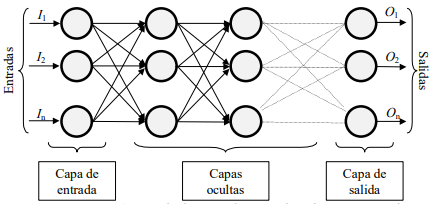
\includegraphics[scale=0.8]{imagenes/rnaBasico.png}
		\caption{Red neuronal artificial.}
		\begin{center}
    Fuente: \cite{redneuronalimagen}.
    \end{center}
	\label{fig:rnaBasico}
\end{figure}

Esta red neuronal está constituida por neuronas interconectadas y arregladas en tres capas. Los datos ingresan por medio de la “capa de entrada”, pasan a través de la “capa oculta” y salen por la “capa de salida”. Cabe mencionar que la capa oculta puede estar constituida por varias capas.

\subsubsection{Función de entrada (input function)}
La neurona trata a muchos valores de entrada como si fueran uno solo; esto recibe el nombre de entrada global. Por lo tanto, ahora nos enfrentamos al problema de cómo se pueden combinar estas simples entradas $(in_{i1}, in_{i2}, ...)$ dentro de la entrada global, $gin_{i}$. Esto se logra a través de la función de entrada, la cual se calcula a partir del vector entrada. La función de entrada puede describirse como sigue:

\begin{equation}
input_{i}=(in_{i1} \bullet w_{i1})\ast (in_{i2} \bullet w_{i2} \ast ... (in_{in} \bullet w_{in})
\end{equation}

donde: $\ast$ representa al operador apropiado (por ejemplo: máximo, sumatoria, productoria, etc.), $n$ al número de entradas a la neurona $n_{i}$ y $w_{i}$ al peso. \citep{matich2001redes}.

\subsubsection{Función de activación (activation function)}
Una neurona biológica puede estar activa (excitada) o inactiva (no excitada); es decir, que tiene un “estado de activación”. Las neuronas artificiales también tienen diferentes estados de activación; algunas de ellas solamente dos, al igual que las biológicas, pero otras pueden tomar cualquier valor dentro de un conjunto determinado. \citep{matich2001redes}.\\
La función activación calcula el estado de actividad de una neurona; transformando la entrada global (menos el umbral, $\sigma_{i}$) en un valor (estado) de activación, cuyo rango normalmente va de (0 a 1) o de (–1 a 1). Esto es así, porque una neurona puede estar totalmente inactiva (0 o –1) o activa (1).
La función activación, es una función de la entrada global ($gin_{i}$) menos el umbral ($\sigma_{i}$). Las funciones de activación más comúnmente utilizadas se detallan a continuación:

\begin{itemize}
\item Función Lineal
\end{itemize}

con $x=gin_{i} -	\sigma, $ y $a >0.$\\
Los valores de salida obtenidos por medio de esta función de activación serán: $a\cdot(gin_{i} - \sigma_{i})$, cuando el argumento de $(gin_{i} - \sigma_{i})$ esté comprendido dentro del rango $(-1/a, 1/a)$. Por encima o por debajo de esta zona se fija la salida en 1 o –1, respectivamente.
Cuando $a = 1$ (siendo que la misma afecta la pendiente de la gráfica), la salida es igual a la entrada. \citep{matich2001redes}.

\begin{itemize}
    \item Función Sigmoidea
\end{itemize}

\begin{equation}
f(x)= \frac{1}{1+e^{-gx}}, \ con \ x=gin_{i}-\sigma,
\label{funcionSigmoidea}
\end{equation}
Los valores de salida que proporciona esta función están comprendidos dentro de un rango que va de 0 a 1. Al
modificar el valor de $g$ se ve afectada la pendiente de la función de activación. 

\begin{figure}[h!]
	\centering
		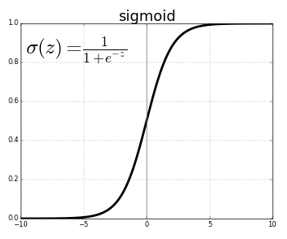
\includegraphics[scale=0.6]{imagenes/Funcionsigmoidea.png}
		\caption{Gráfico de la función sigmoide.}
		\begin{center}
    Fuente: Elaboración propia.
    \end{center}
	\label{fig:Funcionsigmoidea}
\end{figure}
\begin{itemize}
    \item Función Tangente hiperbólica
\end{itemize}

\begin{equation}
f(x)= \frac{e^{gx}-e^{-gx}}{e^{gx}+e^{-gx}}, con x=gin_{i}-\sigma,
\end{equation}
Los valores de salida de la función tangente hiperbólica están comprendidos dentro de un rango que va de -1 a 1. Al modificar el valor de $g$ se ve afectada la pendiente de la función de activación. 

\subsubsection{Función de salida (output function)}
El último componente que una neurona necesita es la función de salida. El valor resultante de esta función es la salida de la neurona $i$ ($out_{i}$); por ende, la función de salida determina que valor se transfiere a las neuronas vinculadas. Si la función de
activación está por debajo de un umbral determinado, ninguna salida se pasa a la neurona subsiguiente. Normalmente, no cualquier valor es permitido como una entrada para una neurona, por lo tanto, los valores de salida están comprendidos en el rango
$[0, 1]$ o $[-1, 1]$. También pueden ser binarios ${0, 1}$ o ${-1, 1}$. \citep{matich2001redes}.

Dos de las funciones de salida más comunes son cuando: la salida es la misma que la entrada (función identidad), o binaria, que devuelve uno cuando el $act_{i}$ es mayor  o igual que el umbral $\epsilon_{i}$, caso contrario es cero. 

\subsection{Perceptrón}
El perceptrón lee los valores de entrada, después suma todas las entradas teniendo en cuenta los pesos y por último el resultado lo introduce en una función de activación que nos genera el resultado final. \citep{perceptron2017}.

\subsubsection{Perceptrón simple}
Se determina los pesos sinápticos y el umbral que proporcione el óptimo ajuste de la entrada con la salida, estas variables, para determinar estas variables se sigue un proceso adaptativo, el cual  comienza con valores aleatorios y se van modificando según la diferencia entre los valores deseados y los calculados por la red.

Recordar que el perceptrón sólo es capaz de representar funciones lineales, dado que no dispone de capas ocultas, para esto existen los perceptrones multicapa.

\begin{table}[h!]
\centering
\caption{Componentes del perceptrón.}
\label{ComponentePerceptron}
\begin{tabular}{|c|l|}
\hline
\rowcolor[HTML]{2E9AFE} 
{\color[HTML]{FFFFFF} \textbf{\begin{tabular}[c]{@{}c@{}}Componentes del\\ perceptrón\end{tabular}}} & \multicolumn{1}{c|}{\cellcolor[HTML]{2E9AFE}{\color[HTML]{FFFFFF} \textbf{Definición}}}                                                                                                                          \\ \hline
\rowcolor[HTML]{81DAF5} 
Entradas                                                                                             & Es la información que recibe el perceptrón.                                                                                                                                                                      \\ \hline
\rowcolor[HTML]{81DAF5} 
Pesos                                                                                                & \begin{tabular}[c]{@{}l@{}}Son los valores numéricos que se encargan de establecer la\\ influencia de una entrada en la salida deseada.\end{tabular}                                                             \\ \hline
\rowcolor[HTML]{81DAF5} 
Bias                                                                                                 & \begin{tabular}[c]{@{}l@{}}Es un parámetro que tienen algunos modelos de redes\\ neuronales el cual permite encontrar fácilmente la\\ separación entre posibilidades de salida de una red neuronal.\end{tabular} \\ \hline
\rowcolor[HTML]{81DAF5} 
\begin{tabular}[c]{@{}c@{}}Función de \\ activación\end{tabular}                                     & \begin{tabular}[c]{@{}l@{}}Se encarga de determinar un valor de salida una\\ vez se han procesado cada una de las entradas.\end{tabular}                                                                         \\ \hline
\end{tabular}
\begin{center}
Fuente: Elaboración propia según \cite{perceptron2017}.
\end{center}
\end{table}
\newpage
En la Tabla \ref{ComponentePerceptron}  se representan los componente del perceptrón simple.

El entrenamiento del perceptrón es un proceso iterativo y sigue los siguientes pasos, hasta lograr reducir el error:
\begin{itemize}
    \item Paso 1: Inicializar los pesos y el bias.
\item Paso 2: Calcular las salidas (net) con los pesos y el bias.
\item Paso 3: Obtener la salida utilizando la función de activación y calcular cada valor del error.
\item Paso 4: Corregir el Bias y los pesos.
\end{itemize}

\subsubsection{Perceptrón Multicapa}
El Perceptrón multicapa es una red de alimentación hacia delante compuesta por una capa de N
neuronas de entrada (sensores), otra capa formada por M neuronas de salida y un número determinado
de capas ocultas. (Ver Figura \ref{Fig:21}). El tamaño de éstas dependerán de la dificultad de la correspondencia
a implementar. \citep{muntintroduccion}.

\begin{figure}[h!]
	\centering
		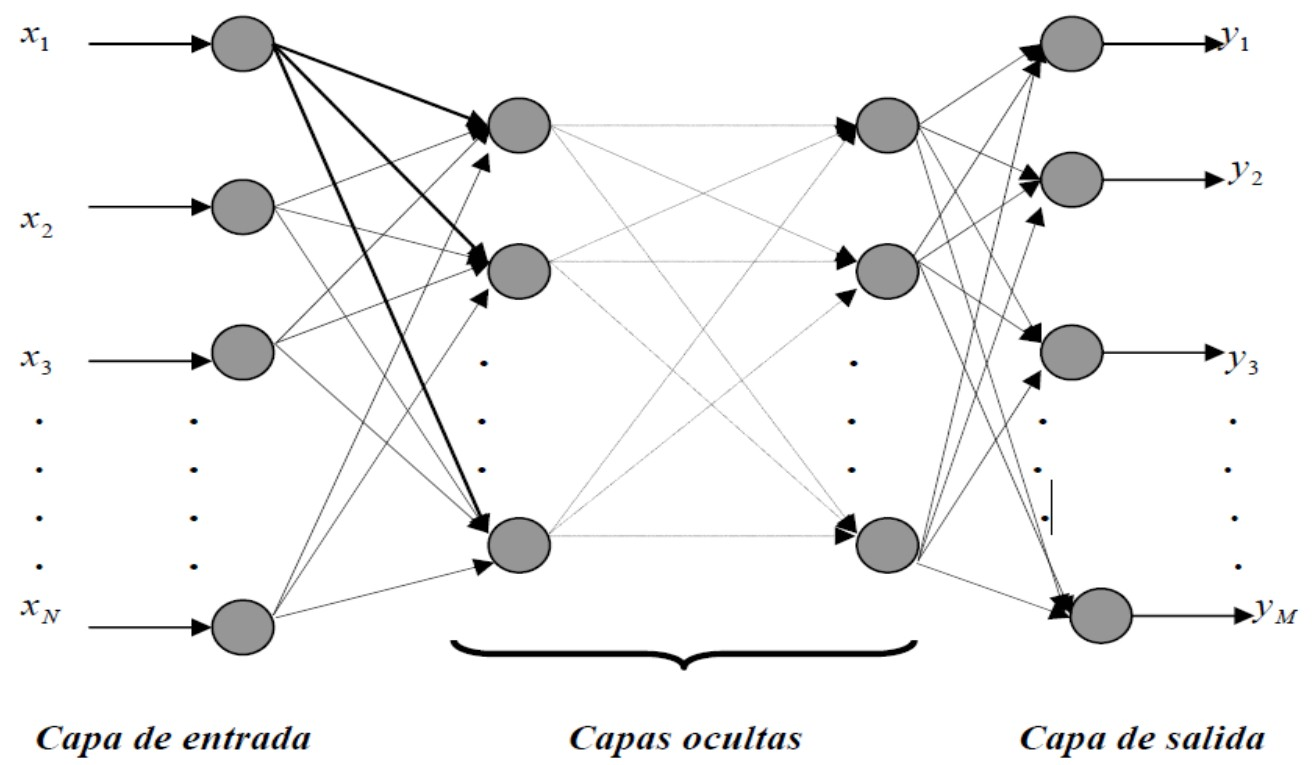
\includegraphics[scale=0.4]{imagenes/perpceMultiCapa.jpg}
		\caption{Representación de un red multicapa.}
		\begin{center}
    Fuente: Alba Morera (2018).
    \end{center}
	\label{Fig:21}
\end{figure}
\newpage
El objetivo que se busca con este tipo de red es el mismo, establecer una correspondencia entre un
conjunto de entrada y un conjunto de salidas deseadas, de manera que:

\begin{equation}
(x_{1},...,x_{n}) \epsilon \mathbb{R}_{N} \rightarrow (y_{1},...,y_{n}) \epsilon \mathbb{R}_{M}
\end{equation}

Para ello se dispone de un conjunto de p pares de entrenamiento de manera que sabemos perfectamente que al patrón de entrada $(x_{1}^{k},...,x_{N}^{k})$ le corresponde la salida $(y_{1}^{k},...,y_{M}^{k}), k = 1,...,p$. Así, nuestro
conjunto de entrenamiento es:
\begin{equation}
{(x_{1}^{k},...,x_{N}^{k}) \rightarrow (y_{1}^{k},...,y_{M}^{k}),k? 1, ..., p}
\end{equation}

\subsection{Backpropagation}
La red neuronal propaga la señal de los datos de entrada hacia adelante a través de sus parámetros hacia el momento de la decisión, y luego propaga hacia atrás la información sobre el error, a la inversa a través de la red, para que pueda alterar los parámetros. Esto sucede paso a paso:
\begin{itemize}
\item La red adivina los datos, utilizando sus parámetros.
\item La red se mide con una función de pérdida.
\item El error se propaga hacia atrás para ajustar los parámetros equivocados.
\end{itemize}

La propagación hacia atrás de errores o retropropagación (del inglés backpropagation) es un método de cálculo del gradiente utilizado en algoritmos de aprendizaje supervisado utilizados para entrenar redes neuronales artificiales. El método emplea un ciclo propagación (adaptación de dos fases). Una vez que se ha aplicado un patrón a la entrada de la red como estímulo, este se propaga desde la primera capa a través de las capas siguientes de la red, hasta generar una salida. La señal de salida se compara con la salida deseada y se calcula una señal de error para cada una de las salidas.

Las salidas de error se propagan hacia atrás, partiendo de la capa de salida, hacia todas las neuronas de la capa oculta que contribuyen directamente a la salida. Sin embargo, las neuronas de la capa oculta sólo reciben una fracción de la señal total del error, basándose aproximadamente en la contribución relativa que haya aportado cada neurona a la salida original. Este proceso se repite, capa por capa, hasta que todas las neuronas de la red hayan recibido una señal de error que describa su contribución relativa al error total.

La importancia de este proceso consiste en que, a medida que se entrena la red, las neuronas de las capas intermedias se organizan a sí mismas de tal modo que las distintas neuronas aprenden a reconocer distintas características del espacio total de entrada. Después del entrenamiento, cuando se les presente un patrón arbitrario de entrada que contenga ruido o que esté incompleto, las neuronas de la capa oculta de la red responderán con una salida activa si la nueva entrada contiene un patrón que se asemeje a aquella característica que las neuronas individuales hayan aprendido a reconocer durante su entrenamiento.

\begin{figure}[h!]
	\centering
		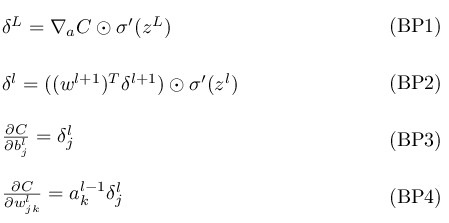
\includegraphics[scale=0.7]{imagenes/ecuacionesBackpropagation.png}
		\caption{Ecuaciones del backpropagation.}
		\begin{center}
    Fuente: \cite{ecuBack}.
    \end{center}
	\label{Fig:ecuacionesBackpropagation}
\end{figure}

Donde: BP1 es para el error en la capa de salida, BP2 es para el error en términos del error en la siguiente capa, BP3 es para la tasa de cambio del costo con respecto a cualquier sesgo en la red y BP4 es para la tasa de cambio del costo con respecto a cualquier peso en la red.

\subsection{Definición de regresión }
Según \cite{pat2013introduccion}, el término de regresión es uno de los pilares estadísticos más modernos el cual hace referencia al análisis simultaneo de dos o más variables relacionadas entre sí.

Una de las variables se le conoce como variable dependiente (y) y la otra como variable independiente (x).

\begin{equation}
    Y=B_{0}+B_{1}X_{1}+B_{2}X_{2}+...+B_{k}X_{k}
\end{equation}

Donde:
$Y$:  es la variable dependiente, la cual también es denominada variable respuesta
$X_{i}$:  es la variable independiente i, la cual también se llama exploratoria
$B_{i}$:  es el coeficiente del modelo para la variable $X_{i}$

Tanto la variable independiente como las independientes deben ser métricas, aunque las independientes también pueden tener valores cualitativos

\subsubsection{Fases del análisis de regresión múltiple}
Según \cite{pat2013introduccion}, las fases son:

\begin{itemize}
    \item Identificar problema o área de oportunidad.
    \item Seleccionar las variables dependientes e independientes.
    \item Recolectar variables.
    \item Realizar análisis descriptivo del tipo de relación entre variables.
    \item Seleccionar método.
    \item Calcular coeficientes del modelo de regresión lineal múltiple para construir la función.
    \item Identificar problemas de colinealidad o multicolinealidad.
    \item Realizar prueba global de la ecuación.
    \item Efectuar pruebas individuales de los coeficientes.
    \item Probar cumplimiento de los supuestos del análisis.
    \item .Interpretar coeficientes de determinación, correlación, determinación ajustado y error estándar.
    \item Analizar los coeficientes de la ecuación de regresión.
    \item Elaborar pronósticos puntuales y por intervalo.
\end{itemize}

\subsection{Python}
Python es un lenguaje de programación interpretado simple pero poderoso que cierra la brecha entre la programación de C y la de shell y, por lo tanto, es ideal para la "programación desechable" y la creación rápida de prototipos. Su sintaxis se construye a partir de construcciones tomadas de una variedad de otros lenguajes; las más destacadas son las influencias de ABC, C, Modula-3 e Icon. El intérprete de Python se puede ampliar fácilmente con nuevas funciones y tipos de datos implementados en C. Python también es adecuado como lenguaje de extensión para aplicaciones C altamente personalizables, como editores o administradores de ventanas. Python está disponible para varios sistemas operativos, entre los que se encuentran varios tipos de UNIX (incluido Linux), el sistema operativo Apple Macintosh, MS-DOS, MS-Windows 3.1, Windows NT y OS / 2. Es conciso, pero intenta ser exacto y completo. La semántica de los tipos de objetos incorporados no esenciales y de las funciones y módulos incorporados se describe en la Referencia de la biblioteca de Python. \citep{rossum1995python}.

\subsection{TensorFlow}
TensorFlow implementa una visión de la teoría de la probabilidad adaptada al paradigma moderno de aprendizaje profundo de computación diferenciable de extremo a extremo. Basado en dos abstracciones básicas, ofrece bloques de construcción flexibles para el cálculo probabilístico. Las distribuciones proporcionan métodos rápidos y numéricamente estables para generar muestras y calcular estadísticas, por ejemplo, densidad logarítmica. Los bijectors proporcionan transformaciones de seguimiento de volumen componibles con almacenamiento en caché automático. Juntos, permiten la construcción modular de distribuciones y transformaciones de alta dimensión que no son posibles con bibliotecas anteriores (por ejemplo, pixelCNN, flujos autorregresivos y redes residuales reversibles). Son el caballo de batalla detrás de los sistemas de programación probabilísticos profundos como Edward y potencian la inferencia rápida de caja negra en modelos probabilísticos construidos sobre componentes de redes profundas.. \citep{dillon2017tensorflow}.

\section{Método de la investigación}
\subsection{Tipo de investigación}
La presente tesis es del tipo experimental.

\subsection{Variables de la Investigación}
\subsubsection{Variable Dependiente}
Pronosticar las ventas en el Mall Aventura Plaza.
\subsubsection{Variable Independiente}
Sistema basado en conocimiento mediante RNA.

\subsection{Operacionalización de la variable}
Nos permiten realizar mediciones y determinar la validez de la hipótesis que fue planteada en la investigación. 

\section{Recolección de datos para la elaboración del modelo}
\subsection{Técnica}
Observación, fue la técnica aplicada para la recolección de datos, específicamente la observación estructurada. Indicando la cantidad de ventas realizadas en la fecha respectiva.

\subsection{Población}
La población para nuestra investigación son las ventas del 2018 hasta el 2020 en el Restaurante Combiche en el Mall Aventura Plaza - Trujillo.

\subsection{Muestra}
Este conjunto de datos está conformado por un dataset de 968 registros, que representan las ventas durante el período enero del 2018 hasta agosto del 2020. Se optó por usar un muestreo aletorio simple  con un nivel de confianza del 95\% y un error de muestreo del 5\%.

\begin{equation}
\label{eq:ecuacion}
n = \frac{z^{2}pq}{e^2}
\end{equation}

En el que:
\begin{enumerate}
\item[•]$n$ = Tamaño de muestra.
\item[•]$z$ = Coeficiente de confiabilidad 95\% al que corresponde (1.96).
\item[•]$pq$ = Varianza de la población, ponemos la varianza mayor posible porque a mayor varianza hará falta una muestra mayor (0.25).
\item[•]$e$ = Error muestral 5\% (0.5).
\end{enumerate}

%Este conjunto de documentos está conformado por una población de 134 documentos, los cuales fueron datos tomados de la recepción en una oficina al azar de la Universidad Nacional de Trujillo, Dirección de Calidad Universitaria, estos documentos fueron editados de tal forma que no permita dar a conocer nombres o datos que podrían ser utilizados con otros fines que no sean de estudio o investigación. Los datos obtenidos fueron:
%\begin{table}[h!]
%\centering
%\caption{Datos obtenidos para la investigación.}
%\label{tab:my-table}
%\begin{tabular}{|l|c|}
%\hline
%\rowcolor[HTML]{2E9AFE} 
%\multicolumn{1}{|c|}{\cellcolor[HTML]{2E9AFE}{\color[HTML]{FFFFFF} \textbf{Día}}}   & {\color[HTML]{FFFFFF} \textbf{Cantidad de documentos}} \\ \hline
%\rowcolor[HTML]{81DAF5} 
%Lunes 26                                                                            & 28                                                     \\ \hline
%\rowcolor[HTML]{81DAF5} 
%Martes 27                                                                           & 31                                                     \\ \hline
%\rowcolor[HTML]{81DAF5} 
%Miércoles 28                                                                        & 22                                                     \\ \hline
%\rowcolor[HTML]{81DAF5} 
%Jueves 29                                                                           & 32                                                     \\ \hline
%\rowcolor[HTML]{81DAF5} 
%Viernes 30                                                                          & 21                                                     \\ \hline
%\rowcolor[HTML]{2E9AFE} 
%\multicolumn{1}{|c|}{\cellcolor[HTML]{2E9AFE}{\color[HTML]{FFFFFF} \textbf{Total}}} & {\color[HTML]{FFFFFF} \textbf{134}}                    \\ \hline
%\end{tabular}
%\begin{center}
%Fuente: Elaboración propia.
%\end{center}
%\end{table}

%\begin{table}[h!]
%\centering
%\caption{Tipos de documentos y sus cantidades.}
%\label{tab:my-table}
%\begin{tabular}{|l|c|}
%\hline
%\rowcolor[HTML]{2E9AFE} 
%\multicolumn{1}{|c|}{\cellcolor[HTML]{2E9AFE}{\color[HTML]{FFFFFF} \textbf{Tipo de documento}}} & {\color[HTML]{FFFFFF} \textbf{Cantidad}} \\ \hline
%\rowcolor[HTML]{81DAF5} 
%Oficio                                                                                          & 54                                       \\ \hline
%\rowcolor[HTML]{81DAF5} 
%Oficio múltiple                                                                                 & 14                                       \\ \hline
%\rowcolor[HTML]{81DAF5} 
%Informe                                                                                         & 24                                       \\ \hline
%\rowcolor[HTML]{81DAF5} 
%Solicitud                                                                                       & 22                                       \\ \hline
%\rowcolor[HTML]{81DAF5} 
%Resolución rectoral                                                                             & 14                                       \\ \hline
%\rowcolor[HTML]{81DAF5} 
%Memorandum                                                                                      & 6                                        \\ \hline
%\rowcolor[HTML]{2E9AFE} 
%\multicolumn{1}{|c|}{\cellcolor[HTML]{2E9AFE}{\color[HTML]{FFFFFF} \textbf{Total}}}             & {\color[HTML]{FFFFFF} \textbf{134}}      \\ \hline
%\end{tabular}
%\begin{center}
%Fuente: Elaboración propia.
%\end{center}
%\end{table}

%\begin{figure}[h!]
%	\centering
%		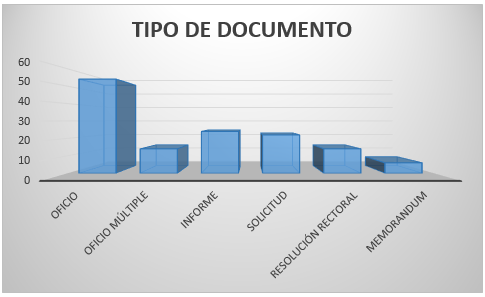
\includegraphics[scale=0.5]{imagenes/RepreGrafica.png}
%		\caption{Diagrama de tipos de documentos.}
%	\begin{center}
%    Fuente: Elaboración propia.
%    \end{center}
%	\label{fig:RepreGrafica}
%\end{figure}
%Estos datos fueron recogidos de la oficina y tienen lugar en el tiempo en la última semana de agosto del 2019.

\section{Etapas de la investigación}
Nuestra investigación comprenderá  las siguientes etapas:
\begin{itemize}
\item La investigación bibliográfica a través de búsqueda de artículos en la web, libros y casos de estudio en relación con el tema de investigación (pronósticos de ventas).
\item La aplicación de la metodología RUP.
\item Recolección de nuestra población, ventas, los cuales se utilizó en el desarrollo de la investigación.
\item Teniendo en cuenta que se necesita entrenar a las redes neuronales, puesto que son  que las redes neuronales son heurísticas se requieren un constante ajuste para obtener un óptimo resultado.
\item Comparar resultados del software con la información del dataset.
\end{itemize}

\chapter{Sistema Basado en Conocimiento Mediante RNA para Pronósticar las Ventas del Restaurante Combiche en el Mall Aventura}
\renewcommand{\baselinestretch}{2} %doble espacio paratodo el texto

\section{Análisis}

\subsection{Requerimiento funcional}
La siguiente imagen (ver Figura: \ref{fig:reqFuncional}) hace referencia y describen las actividades del sistema.

\begin{figure}[h!]
	\centering
		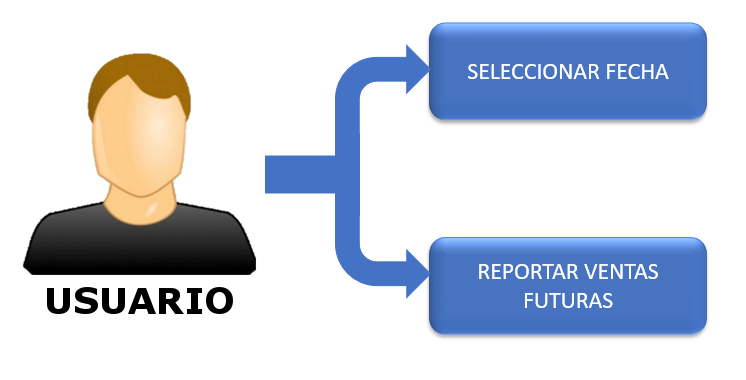
\includegraphics[scale=0.7]{imagenes/requerimientos.png}
		\caption{Requerimiento funcional de investigación.}
	\begin{center}
    Fuente: Elaboración propia.
    \end{center}
	\label{fig:reqFuncional}
\end{figure}
\newpage
Usuario: 
\begin{itemize}
    \item Seleccionar la fecha a pronósticar.
    \item Reportar futuras ventas gráficamente.
\end{itemize}

\subsection{Requemiento no funcional}
Describe otras prestaciones, características y/o limitaciones del sistema.

\begin{table}[h!]
\centering
\caption{Requerimiento no funcional del sistema.}
\label{tab:my-table}
\begin{tabular}{|c|l|}
\hline
\rowcolor[HTML]{aeb6b6} 
{\color[HTML]{FFFFFF} \textbf{Requerimiento no funcional}} & \multicolumn{1}{c|}{\cellcolor[HTML]{aeb6b6}{\color[HTML]{FFFFFF} \textbf{Descripción}}} \\ \hline
\rowcolor[HTML]{ededed} 
\textbf{Usabilidad} & \begin{tabular}[c]{@{}l@{}}Aplicación de fácil manejo, con interfaz gráfica sencilla.\end{tabular} \\ \hline
\rowcolor[HTML]{ededed} 
\textbf{Eficiencia} & \begin{tabular}[c]{@{}l@{}}Aplicación eficiente, ligera y con respuesta rápida.\end{tabular} \\ \hline
\rowcolor[HTML]{ededed} 
\textbf{Dependibilidad} & \begin{tabular}[c]{@{}l@{}}Aplicación disponible.\\ Aplicación confiable.\\ Aplicación integro, sin alteraciones.\\ Fácil mantenimiento de la aplicación.\end{tabular} \\ \hline
\end{tabular}
\begin{center}
    Fuente: Elaboración propia.
\end{center}
\end{table}

\section{Diseño}
\subsection{Diagrama de clases}
Modelo el cual seguiremos en el desarrollo del sistema.

\begin{figure}[h!]
	\centering
		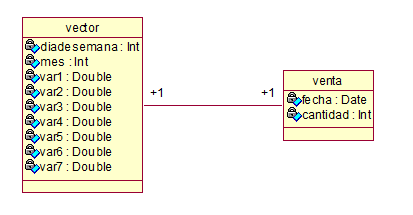
\includegraphics[scale=0.7]{imagenes/diagramaclases.png}
		\caption{Modelo de diagrama de clases para la investigación de la tesis.}
	\begin{center}
    Fuente: Elaboración propia.
    \end{center}
	\label{fig:diagramaClasesTesis}
\end{figure}
\newpage
\subsection{Diagrama de modelos de estados}
Modelo de estados el cual seguiremos en el desarrollo del sistema.

\begin{figure}[h!]
	\centering
		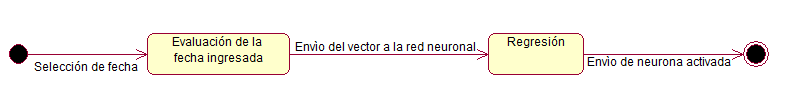
\includegraphics[scale=0.7]{imagenes/modeloestados.png}
		\caption{Modelo de estados para la investigación de la tesis.}
	\begin{center}
    Fuente: Elaboración propia.
    \end{center}
	\label{fig:ModeloEstado}
\end{figure}

\subsection{Diagrama de casos de uso}
Modelo de caso de uso.

\begin{figure}[h!]
	\centering
		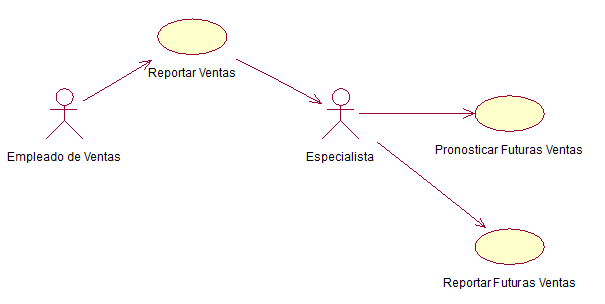
\includegraphics[scale=0.7]{imagenes/usecase.png}
		\caption{Modelo de casos de uso para la investigación de la tesis.}
	\begin{center}
    Fuente: Elaboración propia.
    \end{center}
	\label{fig:diagramaCasosUsoTesis}
\end{figure}
\begin{itemize}
    \item Reportar Ventas, el usuario reporta las ventas a un especialista.
    \item Pronosticar Futuras Ventas, el especialista pronostica las futuras ventas a partir de los reportes.
    \item Reportar Futuras ventas, el especialista brinda el pronóstico de las futuras ventas en un reporte.
\end{itemize}

\subsection{Diagrama de casos de uso del negocio}
Modelo de caso de uso de negocio.

\begin{figure}[h!]
	\centering
		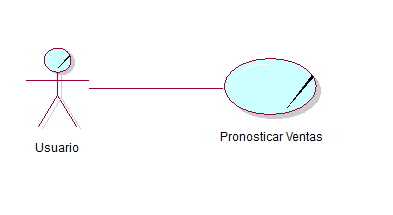
\includegraphics[scale=0.7]{imagenes/casosdeusonegocio.png}
		\caption{Modelo de casos de uso para la investigación de la tesis.}
	\begin{center}
    Fuente: Elaboración propia.
    \end{center}
	\label{fig:diagramaCasosUsoTesis}
\end{figure}
\begin{itemize}
    \item Pronosticar Ventas, El usuario pronostica directamente las futuras ventas mediante un sistema basado en conocimiento.
\end{itemize}

\subsection{Diagrama de componentes}
\begin{figure}[h!]
	\centering
		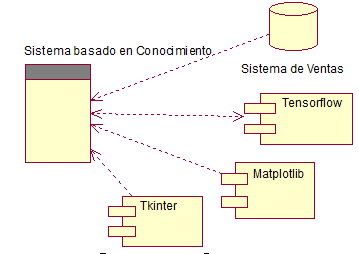
\includegraphics[scale=1]{imagenes/diagramacomponentes.png}
		\caption{Diagrama de componentes de nuestra investigación.}
	\begin{center}
    Fuente: Elaboración propia.
    \end{center}
	\label{fig:diagramadecomponentes}
\end{figure}
\newpage
\subsection{Diagrama de secuencia}
\begin{figure}[h!]
	\centering
		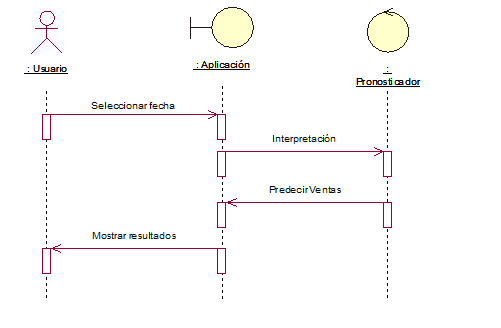
\includegraphics[scale=1]{imagenes/diagramasecuencia.png}
		\caption{Modelo de secuencia para clasificar automáticamente documentos.}
	\begin{center}
    Fuente: Elaboración propia.
    \end{center}
	\label{fig:dsecuencia222}
\end{figure}
\newpage


%\section{Diseño}
\subsection{Diseño de interfaces}
A continuación se muestran la interfaz del sistema:

En la Figura \ref{fig:InterfazAppCap3}, se muestra la ventana principal.

\begin{figure}[h!]
	\centering
		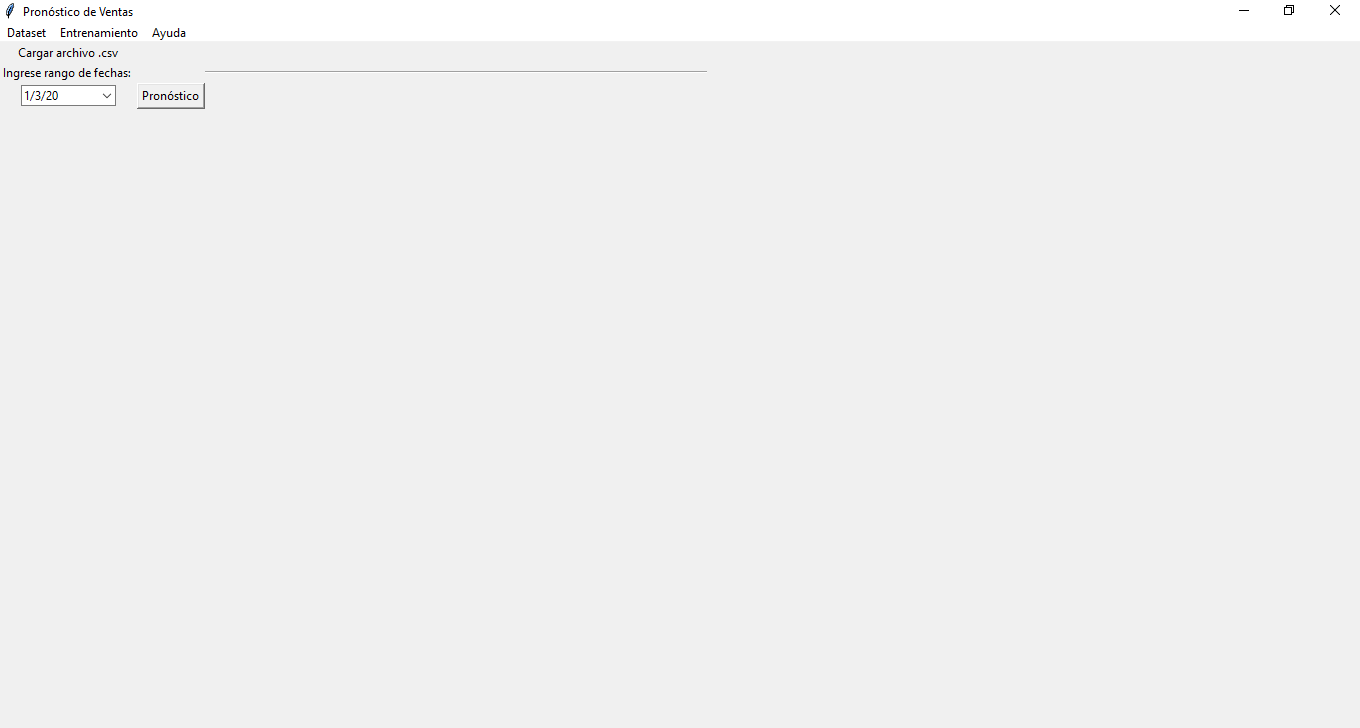
\includegraphics[scale=0.43]{imagenes/mainwindow.png}
		\caption{Ventana Principal del Sistema.}
		\begin{center}
    Fuente: Elaboración propia.
    \end{center}
	\label{fig:InterfazAppCap3}
\end{figure}

\newpage

\subsection{Diseño de algoritmo}

El siguiente diagrama de flujo en el cual mostramos el proceso de implementación computacional que seguimos para el desarrollo.

\begin{figure}[H]
	\centering
		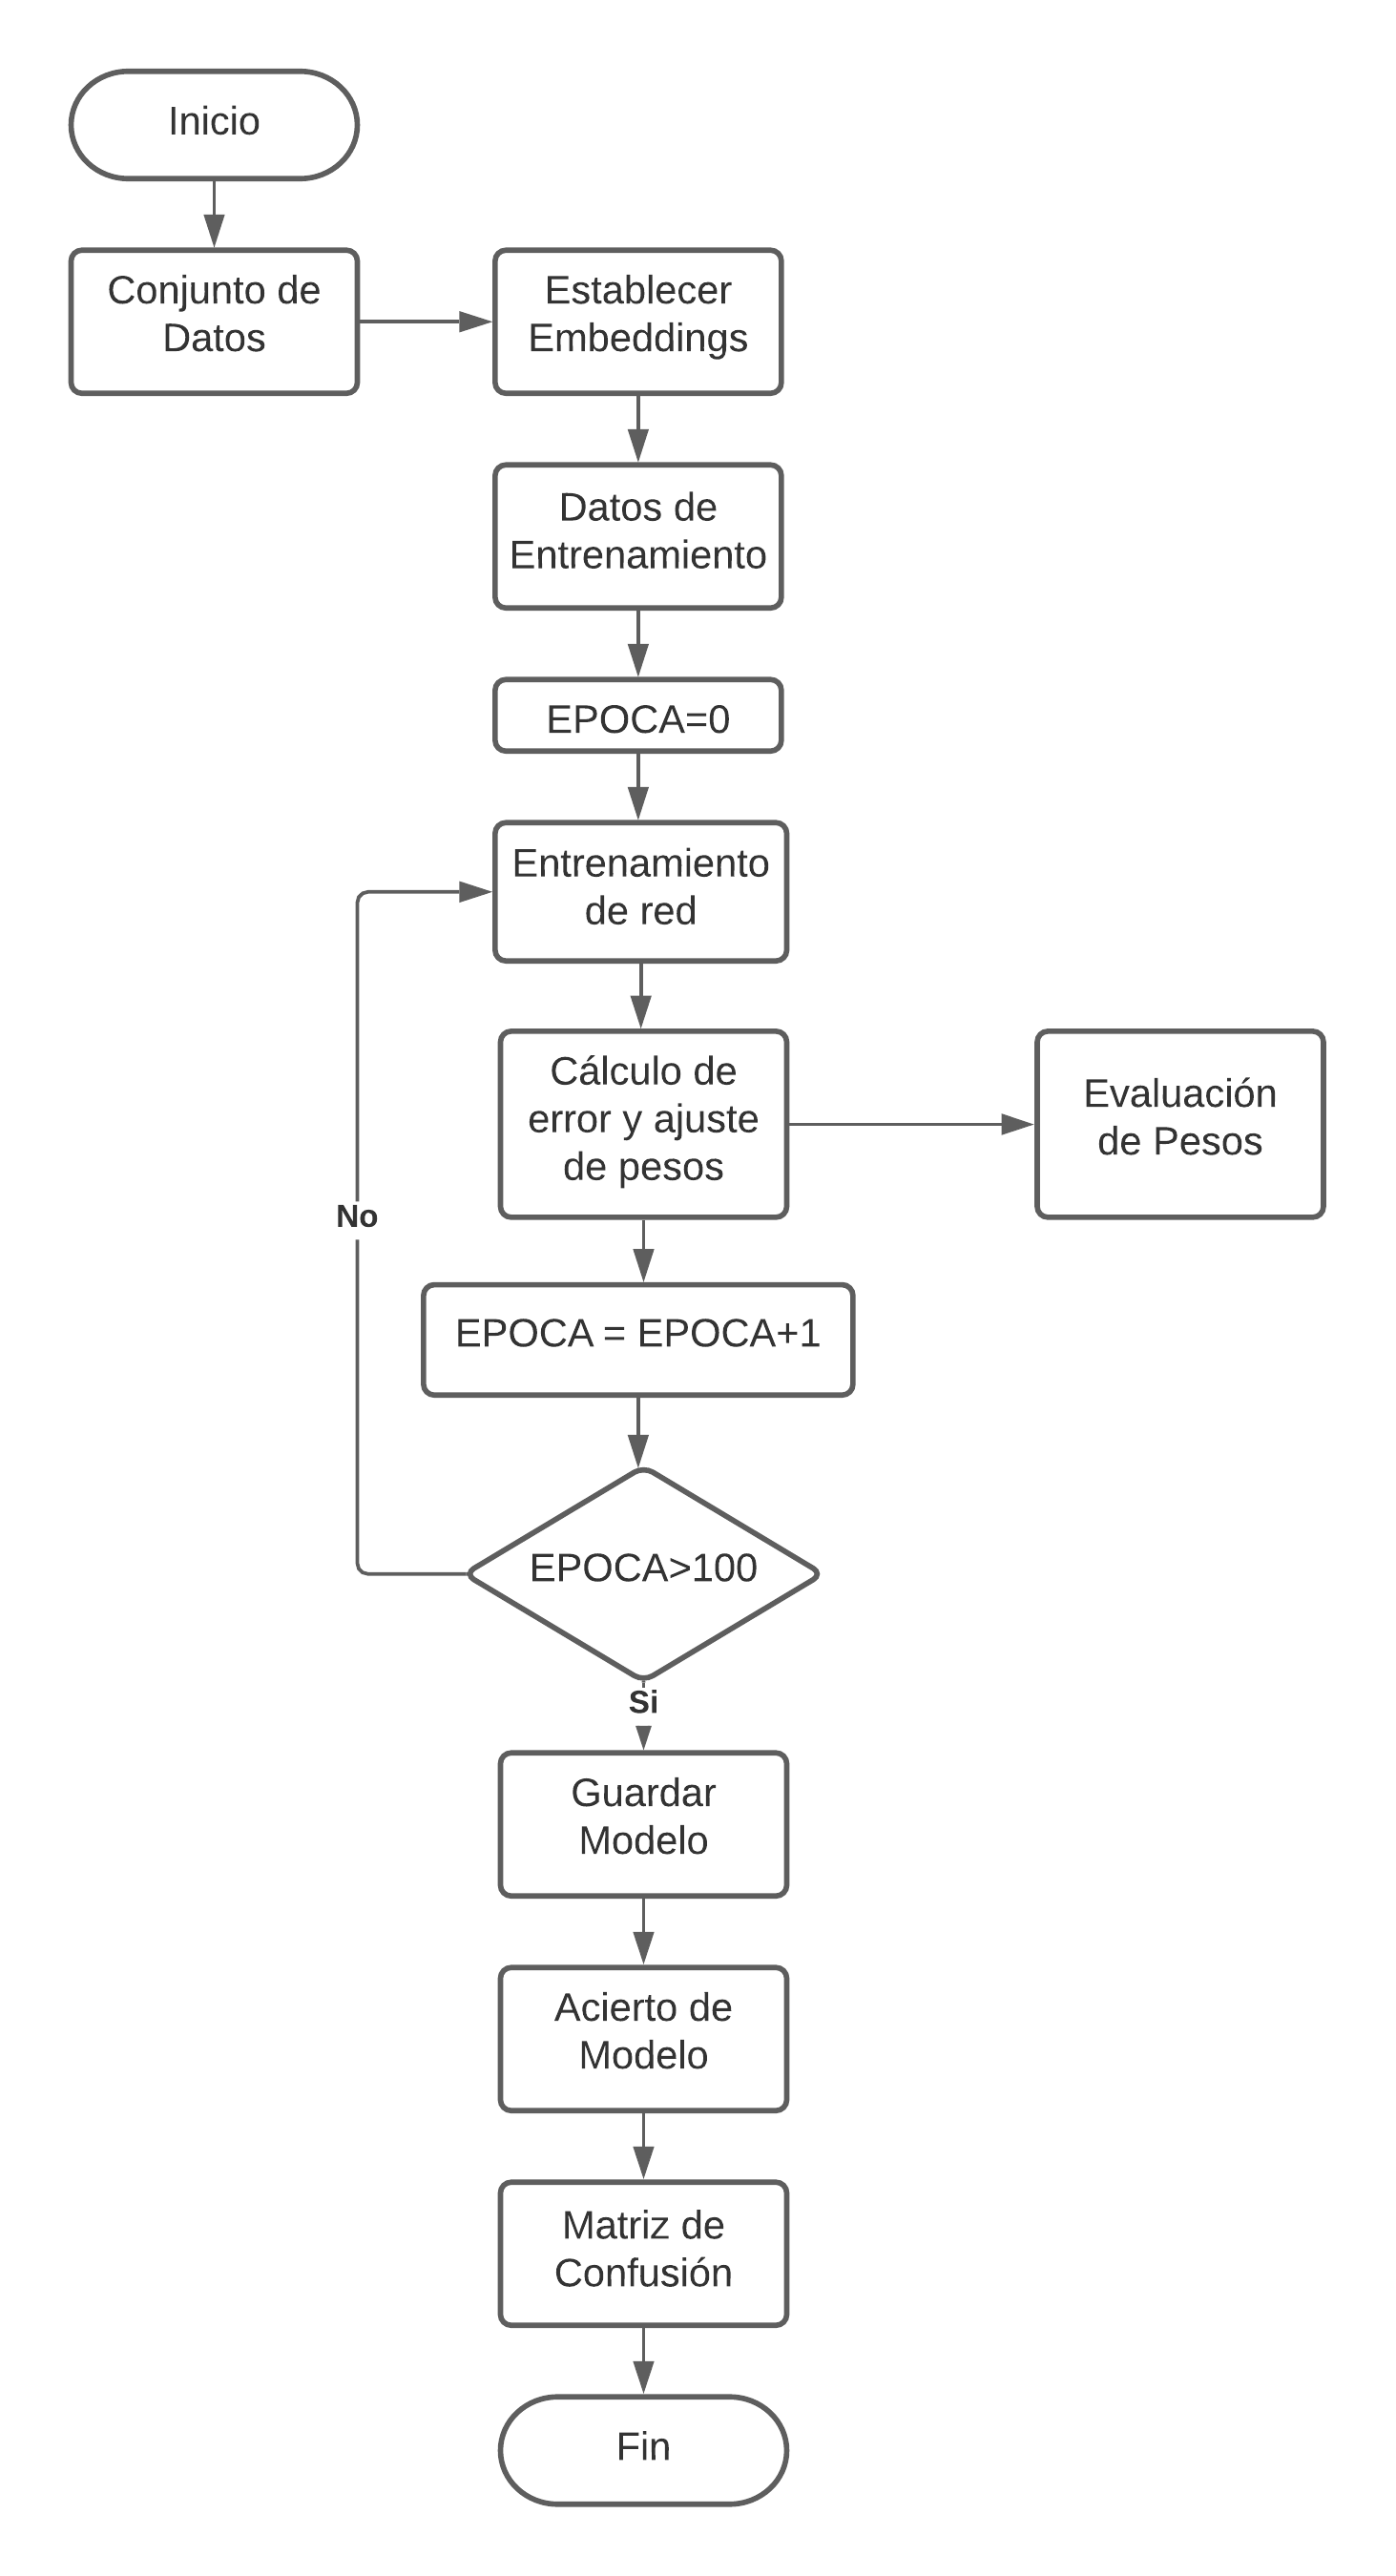
\includegraphics[scale=0.45]{imagenes/flujograma.png}
		\caption{Diagrama de flujo para el desarrollo de la investigación.}
	\begin{center}
    Fuente: Elaboración propia.
    \end{center}
	\label{fig:39}
\end{figure}

\newpage

\subsection{Diseño de Red Neuronal}

El siguiente gráfico es el modelo de neurona utilizada en la red neuronal de la investigación.


\begin{figure}[H]
	\centering
		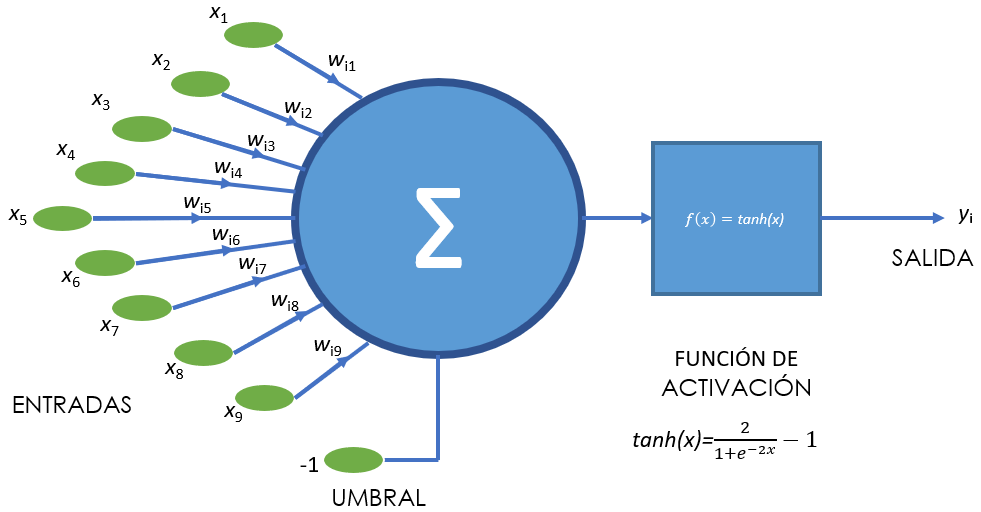
\includegraphics[scale=0.42]{imagenes/modeloneurona.png}
		\caption{Red Neuronal utilizada en la investigación.}
	\begin{center}
    Fuente: Elaboración propia.
    \end{center}
	\label{fig:modelneurona}
\end{figure}


\begin{figure}[H]
	\centering
		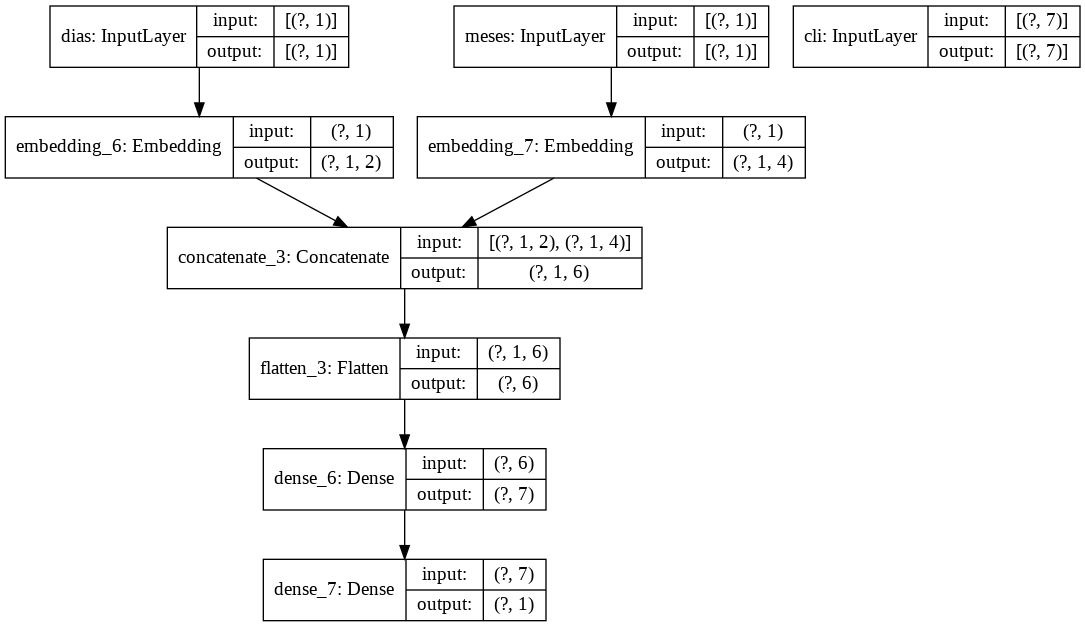
\includegraphics[scale=0.42]{imagenes/neuralnetwork.png}
		\caption{Red Neuronal utilizada en la investigación.}
	\begin{center}
    Fuente: Elaboración propia.
    \end{center}
	\label{fig:neuralnetwork}
\end{figure}

\newpage
\subsection{Extracción de datos}
\begin{figure}[h!]
	\centering
		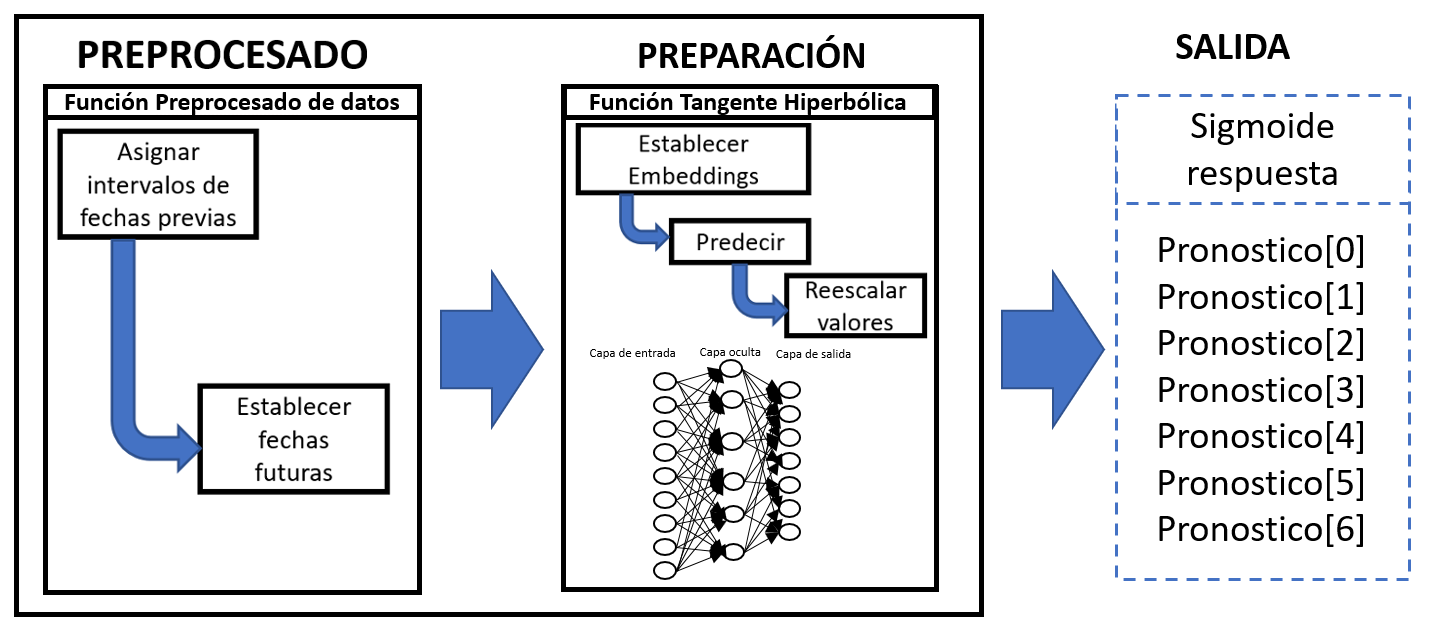
\includegraphics[scale=0.4]{imagenes/extracciondatos.png}
		\caption{Extracción de datos.}
	\begin{center}
    Fuente: Elaboración propia.
    \end{center}
	\label{fig:extracciondedatos}
\end{figure}

Preprocesado:
Selección de las fechas previas(15 días) a la fecha que se quiere pronosticar, de esta manera se tiene los valores de ventas previas a dicha semana, se prepara las fechas futuras(1 semana) a partir de la fecha seleccionada.

Preparación:
Usando los valores de ventas y fechas se le establece sus respectivos valores de Embeddings, se re-escalan los valores para luego predecir en la red neuronal pre-entrenada y se re-escala los valores obtenidos.

Salida:
La función tangente hiperbólica nos da como respuesta un vector, el cual indica los valores de las ventas en la próxima semana iniciando en la fecha indicada.

\begin{figure}[h!]
	\centering
		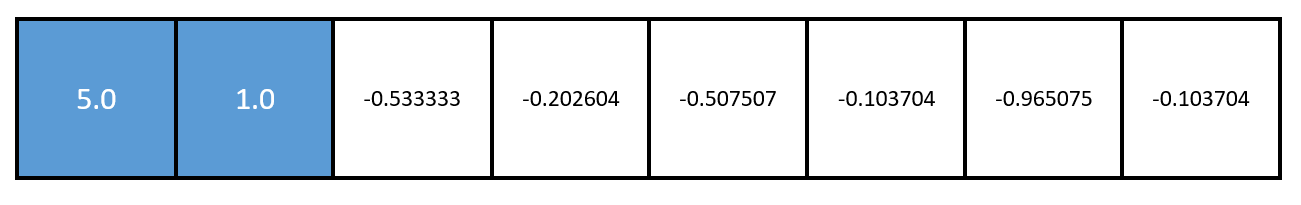
\includegraphics[scale=0.4]{imagenes/vectorcaracteristico.png}
		\caption{Descripción del patrón.}
	\begin{center}
    Fuente: Elaboración propia.
    \end{center}
	\label{fig:DescriPatron}
\end{figure}
En este vector se puede visualizar que los primeros dos valores son extraídos del día de la semana y el mes de la fecha, mientras que los otros siete indican los valores de las fechas siguiente pero re-escalado.
\subsection{Arquitectura de la aplicación}
\begin{figure}[h!]
	\centering
		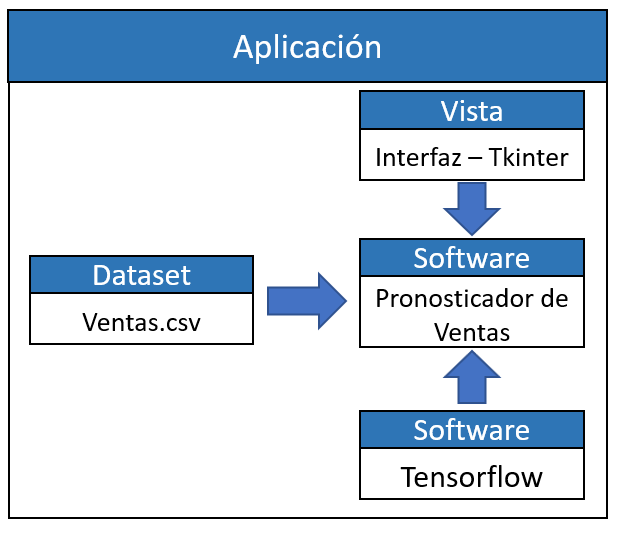
\includegraphics[scale=0.4]{imagenes/arquitecturaaplicacion.png}
		\caption{Arquitectura de la aplicación.}
	\begin{center}
    Fuente: Elaboración propia.
    \end{center}
	\label{fig:arquitecturaaaa}
\end{figure}

\section{Implementación}
Nos enfocamos en la resolución de la tesis y el desarrollo del sistema basado en conocimiento, un software realizado en python independiente de la IDE, usando tensorflow para el entrenamiento y predicción de la red neuronal feedforward, el cual nos mostrará los resultados óptimos de nuestra pronóstico a través de nuestro sistema. \\

En el proceso de entrenamiento de la red neuronal se hizo un total de 100 épocas. Los datos utilizados fueron extraídos de la base de datos del restaurante Combiche en el Mall Aventura y almacenados en un dataset (en formato .csv).


\section{Funcionamiento de las redes neuronales}
Al seleccionar la fecha, se establece vectores de fechas previas para predecir la semana siguiente, se establecen embeddings y se interpreta en la red neuronal.
Los vectores que se obtienen en la prediccion son re-escalados para poder entenderlos.

\newpage
\section{Función activación}
Las redes neuronales feedforward tienen la característica de ir hacia adelante, no presentan bucles. La función de activación nos indica el valor de venta de la fecha siguiente a las fechas ingresadas. Considerando que dicho valor aún necesita re-escalarse.
\newpage

\section{Funciones del sistema:}

Una de las funciones es mostrar gráficamente la pérdida(valores de la función de coste con los datos de entrenamiento).\\
Además, reporta gráficamente los valores de testing y el pronóstico para las fechas a probar.\\
Principalmente, muestra gráficamente los valores del pronóstico de la semana de la fecha seleccionada.

\section{Código Fuente:}

\lstinputlisting[language=Matlab,
    basicstyle=\footnotesize,
    numbers=left,
    stepnumber=1,
    showstringspaces=false,
    tabsize=1,
    breaklines=true,
    breakatwhitespace=false,]{./main.py}

\newpage


\chapter{Resultados y discusión de la tesis}

En la aplicación del sistema basado en conocimiento conseguimos resultados esperados que van de acuerdo con la hipótesis planteada.


\section{Resultados computacionales}

La presente investigación tiene como finalidad pronósticar las ventas de la siguiente semana utilizando un set de datos que entrena a una red neuronal fast forward en un sistema basado en conocimiento. Se consultó el pronóstico para la semana del 23 de febrero del 2020, tomando en cuenta que es semanas antes de la cuarentena.\\
En la tabla 4.1 se muestra el dataset con los valores de venta observados y la fecha, además de una columna con los valores de venta pronosticados por el sistema basado en conocimiento.\\


\begin{table}[h!]
\centering
\begin{tabular}{|l|l|l|l|l|} 
\hline
\textbf{AÑO} & \textbf{MES} & \textbf{DIA} & \textbf{VENTAS OBSERVADAS} & \textbf{PREDICCION}  \\ 
\hline
2020         & 2            & 23           & 5                          & 1                    \\ 
\hline
2020         & 2            & 24           & 0                          & 5                    \\ 
\hline
2020         & 2            & 25           & 16                         & 7                    \\ 
\hline
2020         & 2            & 26           & 5                          & 5                    \\ 
\hline
2020         & 2            & 27           & 3                          & 3                    \\ 
\hline
2020         & 2            & 28           & 2                          & 4                    \\ 
\hline
2020         & 2            & 29           & 5                          & 5                    \\
\hline
\end{tabular}
\end{table}


\section{Discusión de Resultados}

Para la contrastación se utilizó el método Chi-Cuadrado. Utilizando la Tabla 4.1, podemos decir:\\

\begin{center}
$df = 6$\\
$Chi-Square = 11.4039$\\
$p-value = 0.0766682$\\
\end{center}

\begin{figure}[H]
	\centering
		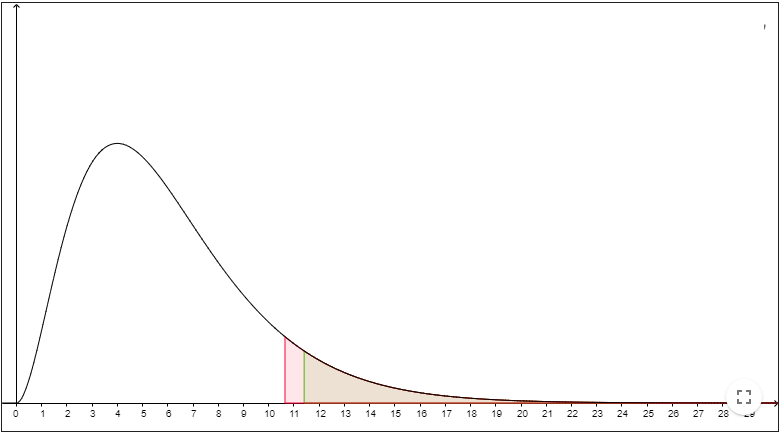
\includegraphics[scale=0.7]{imagenes/chicuadrado.png}
		\caption{Contrastación por método de Chi-Cuadrado en Geogebra.}
	\begin{center}
    Fuente: Elaboración propia.
    \end{center}
	\label{fig:39}
\end{figure}

Con los resultados obtenidos por la contrastación, se obtiene el p-value = 0.0766682, valor inferior a 0.1 por lo tanto, llegamos a la conclusión que la hipótesis es estadisticamente significativa.


\newpage

\chapter{Consideraciones finales}


\section{Conclusiones}

Al finalizar la investigación se pudo cumplir con los objetivos específicos propuestos, los cuales se detallan acontinuación:
\begin{enumerate}
\item Durante esta investigación se pudo explicar la problemática de la pronosticación de ventas así como su solución aplicando un sistema basado en conocimiento, para este caso se determinó usar redes neuronales fast forward, la cual nos permitió pronosticar las ventas de la próxima semana.
\item Se cumplió con la implementación de un prototipo del sistema basado en conocimiento para pronósticos, la cual es muy útil para la toma decisiones.
\item En la investigación se logró descartar la hipótesis nula con un nivel de significancia del 90\%.
\end{enumerate}

\section{Trabajos futuros}

Si bien esta investigación cumple con la hipótesis y objetivos específicos planteados, durante la presente tesis, se presentaron algunas ideas que podrían mejorar la aplicación, por ejemplo:

\begin{itemize}
\item Utilizar datasets con una mayor cantidad de registros, para un mejor entrenamiento de la red neuronal y así una obtener una predicción más eficaz.
\item Proponer automatización del sistema o módulo de compras al conectarlo con el sistema basado en conocimiento para establecer las compras que se realizaran para esa semana de acuerdo a las ventas pronósticadas.
\item Crear un app móvil para acceder al sistema basado en conocimiento de manera remota.
\end{itemize}



\cleardoublepage
\renewcommand\bibname{Referencias bibliográficas}
\addcontentsline{toc}{chapter}{ Referencias bibliográfícas}
\bibliographystyle{apalike}   % estilo de la bibliografía APA.
\bibliography{Bibliografia}   % Archivo de Bibliografia.bib.

